\chapter{Machine Learning} \label{ml}

Machine Learning (ML) is a subfield of Artificial Intelligence (AI). AI is not strictly defined, as the Intelligence itself is not strictly defined. The strict definition of these terms tends to drift more to the field of philosophy than to the field of computer science.\cite{wang2019defining}

Simply put, machine learning is a method to learn to do certain tasks based on data. Machine learning algorithms build models by recognizing and extracting patterns from given training data. Machine learning can be divided into three main types; Supervised Machine Learning, Unsupervised Machine Learning and Reinforcement Learning. Deep learning can be seen as a fourth type of machine learning, that can use techniques from other types of machine learning.\cite{alpaydin2020introduction}

A machine learning model is a mathematical function that is created through the process of training a machine learning algorithm on a given dataset. It captures patterns, relationships, or dependencies in the data and is used for making decisions, predictions, classifications, or other ML operations. ML model can be seen as a `learned' version of the ML algorithm that can generalize from the training data to make predictions or decisions on new, similar data.

\section{Introduction to Artificial Intelligence} \label{ai}

One common and perhaps one of the simplest definitions of Artificial Intelligence is that a machine possesses it when it has the ability to solve hard problems. A more specific, common definition is that AI is a multidisciplinary field, combining computer sciences, mathematics and cognitive sciences, that focuses on developing intelligent machines capable of performing tasks that typically require human intelligence.\cite{nilsson2009quest}

Artificial intelligence can perform a wide range of tasks, such as:

\begin{itemize}
  \item \textbf{Prediction and Classification:} AI can analyze data to make predictions or classify instances into different categories. Machine learning is usually used for prediction and classification. Example prediction tasks can be predicting stock prices or car fuel consumption and diagnosing diseases. Classification can be used for tasks such as spam filtering and customer segmentation.
  \item \textbf{Natural Language Processing (NLP):} NLP is used to enable machines to interpret and generate human language. NLP is used in speech recognition, machine translations and chatbots.
  \item \textbf{Robotics:} AI can help robots to be capable of perceiving their environment, plan actions based on that, and interacting with humans and other machines. Tasks usually done by intelligent robots are, for example, autonomous navigation, human-robot interaction and industrial automation.
  \item \textbf{Computer Vision:} AI can be used to analyze visual data to extract information and interpret the content. Computer vision can be used in object detection, image recognition and facial recognition. Computer vision is a vital part of helping robots to perceive their environment.
  \item \textbf{Recommendation Systems:} AI-based recommendation systems can analyze user behavior and preferences to provide personalized advertisements and recommendations. Recommendation systems are used, for example, in e-commerce sites and streaming platforms.
  \item \textbf{Data-driven decision-making:} AI can be used to discover meaningful patterns, such as trends and insights, from large datasets. This is usually called pattern recognition.
  \item \textbf{Optimization and Planning:} AI can be used to plan strategies to solve complex optimization problems such as route planning, scheduling, supply chain management and resource allocation. 
  \item \textbf{Generation:} Generative AI can be used to generate new content such as images, art, music and written text. Generated text can be written in human language or programming language. Tools made by OpenAI, such as DALL-E and ChatGPT, have lately got a lot of media coverage, and have already been transforming fields like software development and copywriting into fields where usage of generative AI tools is a necessary part of the creation process.
\end{itemize}

\begin{figure}
\centering 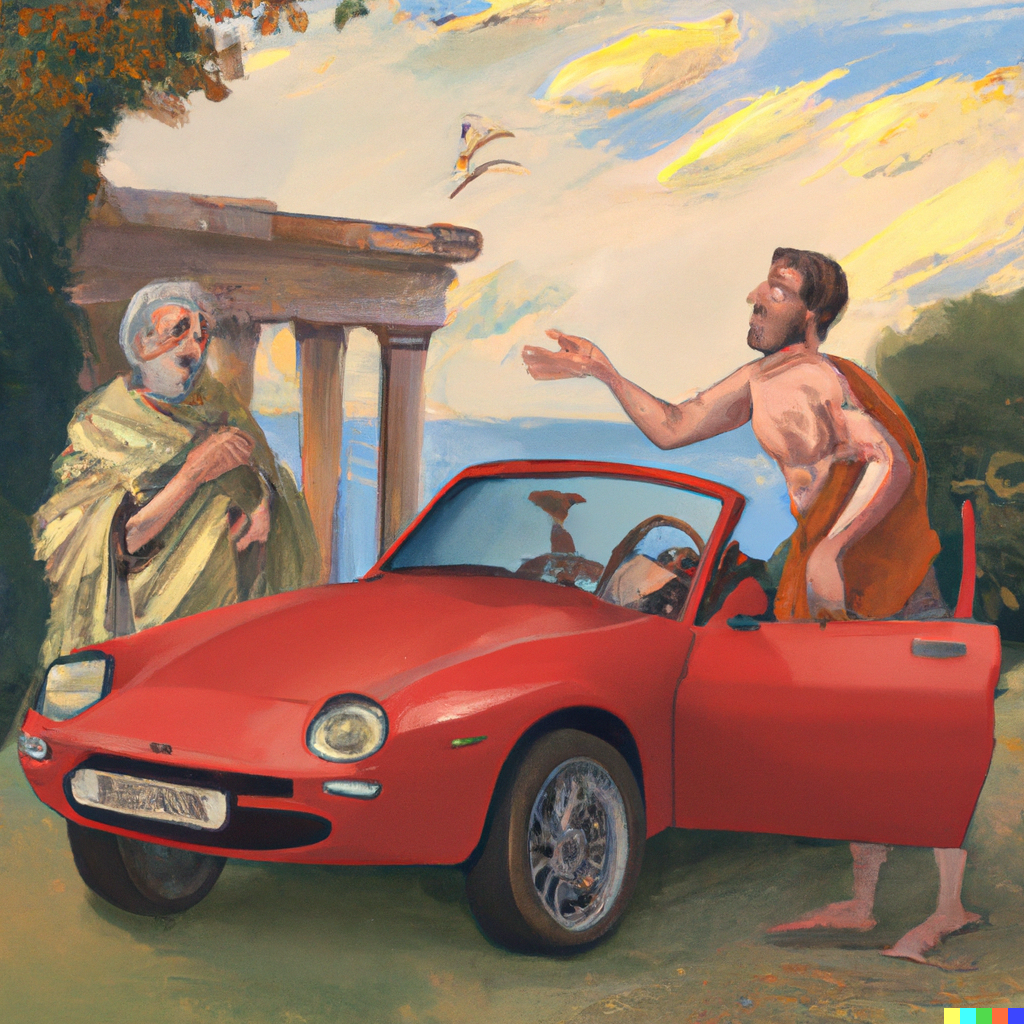
\includegraphics[width=0.5\textwidth]{img/dalle}
\caption{Example of an image generated by DALL-E, when it is asked to generate a painting where Socrates admires Mazda Miata in Ancient Greece.}
\label{img:dalle} 
\end{figure}

Artificial Intelligence can be divided into different types or categories in many ways. Dividing AI into weak or narrow AI and strong AI is a popular high-level way to categorize different Artificial Intelligence methods. In this model, weak AI is AI that is designed to solve specific problems. If the weak AI is given a problem outside the original scope, the weak AI cannot produce reliable results. On the other hand, strong AI is a general-purpose AI that can learn like humans do. Currently, all AI solutions are weak Artificial Intelligences.

Another common high-level way to categorize AI's is to divide them into four different categories; Basic AI, Limited AI, Advanced AI and Superintelligence.

\begin{itemize}
  \item \textbf{Basic AI:} Being the simplest form of AI, the basic AI does not involve any kind of learning. It uses static algorithms, like search algorithms, to produce results.
  \item \textbf{Limited AI:} Limited AI produces results based on a substantial amount of data. Limited AI can learn based on data and produce results by analyzing that data. Machine learning falls into this category.
  \item \textbf{Advanced AI:} Advanced AI has the same intelligence as humans has. Advanced AI can be considered as a general-purpose AI. 
  \item \textbf{Superintelligence:} Superintelligence far surpasses human intelligence.
\end{itemize}

In the context of this thesis, it is perhaps more beneficial to categorize AI based on implementation details. Artificial intelligence solutions have been implemented with different methods throughout the history of AI\cite{russell2010artificial}, such as:

\begin{itemize}
  \item \textbf{Search Algorithms:} Algorithms that can solve many problems by intelligently searching through many possible solutions. Common search algorithms include breadth-first search, depth-first search, A* search, and heuristic-based algorithms. Search algorithms are rarely sufficient for real-world problems, as the number of places to search quickly grows too high.
  \item \textbf{Logic Programming:} AI approach that uses mathematical logic to reason. Rules are specified in the formal logic language.
  \item \textbf{Probabilistic methods for uncertain reasoning:} Probabilistic methods are used to solve the problem when an agent has to act based on uncertain data, using methods from probability theory and economics. Bayesian networks, Markov decision processes, and hidden Markov models are examples of probabilistic methods.
  \item \textbf{Machine Learning:} a subfield of AI that is discussed extensively in this chapter.
  \item \textbf{Artificial Neural Networks (ANNs):} ANNs are models that mimic the functioning of the biological neural networks. ANNs used extensively in deep learning. Examples of artificial neural networks are deep neural networks, convolutional neural networks (CNNs), recurrent neural networks (RNNs), and self-organizing maps (SOMs).
\end{itemize}

\section{Types of Machine Learning} \label{mltypes}

There are four main types of machine learning: supervised learning, unsupervised learning, reinforcement learning and deep learning. Each type has its own characteristics, techniques, and applications. The appropriate type depends on the specific problem, available data, and the desired learning outcome.\cite{burkov2019hundred} 

\subsection{Supervised Machine learning} \label{sml}

The basic idea of Supervised Machine Learning is to predict unknown variables based on known variables. The unknown variable that ML model tries to predict can be a categorical target variable or a numerical target variable. Based on the types of target variables, there are two types of problems in the domain of Supervised Machine Learning; classification problems and regression problems. Training data containing the target variables is called labeled data.

In a classification problem, a supervised ML model tries to predict an unknown category (class label) based on known variables. Classification problems with only two possible outcomes are solved with binary classifiers. This is the case when trying to predict whether a given object is something or not (for example, is this email message spam or not). If there are multiple possible outcomes, then multiclass classifiers are used. In these cases, the model tries to predict the category of a given object (for example, which fruit this fruit is).

In a regression problem, a supervised ML model tries to predict a numerical value for a target variable based on known variables. For example, the model might try to predict the value of real estate based on living area, age, region, etc. of the real estate.

The training dataset consists of instances of data points. Each data point has feature variables (for example, living area, age and region of a real estate) and the target variable (for example, price of the real estate). Data having a target variable called labeled data. When the model is trained, it can be used to predict target variables based on feature variables.

The provided known target variables are what makes supervised machine learning `supervised'.\cite{ml}

\subsection{Unsupervised Machine Learning} \label{usml}

Unlike Supervised Machine Learning, the Unsupervised Machine Learning does not require target variables, so it can operate on unlabeled data. The goal of unsupervised ML is not to predict certain values based on known values, but to find hidden patterns or categorizations in given data.

There is also a type of machine learning that combines techniques from supervised and unsupervised machine learning, called Semi-Supervised Machine Learning.

\subsection{Reinforcement Learning} \label{rl}

Reinforcement Learning learns optimal behaviors through trial and error interactions with an environment. The agent receives feedback in the form of rewards and penalties, and then tries to perform actions that maximize the reward feedback. Reinforcement learning is often used for tasks where an agent learns to take actions to maximize cumulative rewards.

\subsection{Deep Learning} \label{dl}

Deep learning is a complex case of machine learning that uses neural network algorithms to produce results. Neural networks try to mimic the human brain structure. A neural network consists of single nodes or neurons that can communicate with other neurons.

In Deep Learning, the neural networks are aggregated into multiple layers. Each layer extracts more and more higher-level information from the data. Deep learning can use both supervised and unsupervised machine learning.

\section{Machine Learning Algorithms} \label{mlalg}

Machine learning algorithms are mathematical models that are used to perform predictions or decisions based on data. Some of the ML algorithms are specific to the specific type of machine learning, while other ML algorithms can be used in different types of machine learning. Each ML algorithm is suited for different tasks and data characteristics\cite{zhou2021machine}. Examples of ML algorithms:

\begin{itemize}
  \item \textbf{Linear Regression:} A regression algorithm and one of the simplest ML algorithms. Linear regression is used for predicting continuous numerical values based on input variables. It fits a linear relationship between the input variables and the target variable. The example implementation described in Section \ref{implementation} uses linear regression.
  \item \textbf{Logistic Regression:} A classification algorithm that predicts the probability of an instance belonging to a particular class using a logistic function.
  \item \textbf{Decision Trees:} An algorithm that partitions the input into hierarchical decision rules. Decision trees can be used in both regression and classification problems. Algorithms which use multiple decision trees ares called Random Forest algorithms.
  \item \textbf{Support Vector Machines (SVM):} SVM aims to find a hyperplane in an N-dimensional space that classifies the data points. \textit{N} represents the number of features. SVM can be used in both regression and classification problems.
  \item \textbf{K-Nearest Neighbors (KNN):} KNN is used to make predictions based on the similarity of input instances to their neighbors. KNN can be used in both regression and classification problems.
  \item \textbf{Naive Bayes:} An algorithm based on Bayes' theorem that can be used for classification problems.
  \item \textbf{Artificial Neural Networks algorithms:} A class of algorithms that is used with artificial neural networks. ANN algorithms try to mimic the structure of biological neural networks.
  \item \textbf{Clustering Algorithms:} A class of similar algorithms that is used for unsupervised learning. Popular clustering algorithms include K-Means, DBSCAN, and Hierarchical Clustering.
  \item \textbf{Reinforcement Learning Algorithms:}  A class of algorithms that is used with reinforcement learning.
\end{itemize}